\documentclass{xduugthesis}
\usepackage{algorithm}
% \usepackage{algorithmic}
\usepackage{algpseudocodex}
\usepackage{graphicx}
\usepackage{subcaption}
\usepackage{caption}
\usepackage{tabularray}
\usepackage{enumitem}
\usepackage{theorem}
\usepackage{siunitx}
\usepackage{amsmath}
\usepackage{amsfonts}
\usepackage{amssymb}
\usepackage{pifont}
\usepackage{physics}
\usepackage{bm}
\usepackage{multirow} 
\usepackage{booktabs}
\usepackage{url}
\xdusetup{
    style = {
        fix-input = true,
        before-skip = {24pt,22pt,22pt,22pt,12pt,12pt},
        after-skip = {24pt,24pt,24pt,24pt,6pt,6pt}
    },
    info = {
    	title = {图像噪声先验学习与去噪方法},
    	author = {李傲},
        department = {人工智能学院},
        major = {人工智能},
        supervisor = {董伟生},
        class-id = {2020039},
        student-id = {20009200077},
        abstract = {chapters/abstract-zh.tex},
        keywords = {物理噪声模型, 标准化流, 噪声先验, 图像盲去噪 },
        abstract* = {chapters/abstract-en.tex},
        keywords* = {Physics-based Noise Modeling, Normalizing Flow, Noise Prior, Blind Denoising},
        bib-resource = {refs/reference.bib},
       % appendix = {chapters/appendix-a.tex},
        acknowledgements = {chapters/acknowledgements.tex}
    }
}

\def\mathbi#1{\textbf{\em #1}} 

\newcommand{\cmark}{\ding{51}}
\newcommand{\xmark}{\ding{55}}

\renewcommand{\algorithmicrequire}{\textbf{Input:}}
\renewcommand{\algorithmicensure}{\textbf{Output:}}
\renewcommand\thesubfigure{\alph{subfigure})}

% \usepackage{mathtools}
% \newtagform{test}[\text]{\text{\small 式~(}}{)}
% \usetagform{test}

\begin{document}
\chapter{绪论}
\section{研究背景及意义}

随着信息化时代的加速发展,图像作为一种高效直观的信息载体,在人类生活的多个方面展示了其独特的重要性。数字图像是图像的信息化形式, 由于其数字化的特性和可被编程的能力而被广泛应用。 然而数字图像在采集、传输、存储、处理以及显示的过程中, 可能由多种因素导致数字图像中出现丢失的、错误的数字信号,与图像想表达的真实信息不符,这种干扰被称之为图像噪声。

图像去噪是任何图像处理流程中的重要组成部分,在许多重要领域都有应用,包括生物医学成像\cite{ctdenoise, eformer}、遥感成像 \cite{hybridhsidenoise, cnnhsidenoise}、暗光摄影成像\cite{eld}、农业图像\cite{鸡儿denoise, 杂交denoise}等。在进行各种类型的更复杂的任务和算法(例如人脸识别\cite{qualnet}、图像分类\cite{ddp, sfdunet}等)之前,去噪通常是预处理数据集的重要步骤。一个好的去噪模型的要求是在去除图像噪点的同时保留边缘、纹理区域和其他图像细节,在消除噪点和保留精细图像细节之间存在着复杂的平衡,这使消除图像中的噪点成为了一个具有挑战性的问题。此外,噪声源的多变性和不可预测性,图像不断增长的分辨率,也都是开发有效降噪算法所面临的挑战。

在进入深度学习的时代之前,许多去噪算法依赖于贝叶斯公式,即对图像噪声先验的依赖。图像噪声先验构成了图像处理整体进展的支柱,这条路径一般称之为传统图像去噪算法。广泛的工作引入了许多性能良好的去噪算法,以及一个计算机视觉中引人注目的的科学领域。但事实上,这些光辉的成就仍使一些研究人员开始考虑“去噪已死”的可能性\cite{去噪已死},似乎现有的解决方案已经触及了可实现的性能上限。然而近年来,深度学习技术的快速发展为图像去噪提供了新的解决方案,其中也包括图像噪声先验的新发展。研究者们通过深度神经网络强大的特征提取和模式识别能力,从大量的图像数据中学习到噪声的分布和特性,从而实现更为准确和自适应的噪声参数估计,进而进一步提升去噪算法的性能。

%从早期的基于$L_2$的正则化开始,到小波域的引入,再到对偏微分方程的部署,这其中一直延续了稀疏编码、基于补丁的方法和低秩结构假设的方法。

随着社会逐渐进入智能化时代,图像作为机器认识世界的眼睛,使得社会对图像质量的要求越来越高,图像去噪技术也被越来越多的应用。因此,本文对基于深度学习的图像噪声先验学习与去噪方法展开更深入的探究,提出去噪效果更优秀的去噪算法具有重要的实际意义与使用价值。

\section{研究现状}

\subsection{噪声先验}

噪声先验学习,即对真实的噪声进行尽可能准确的建模,从而获得噪声的先验知识。现有的噪声建模方法主要分为两类:一种是基于物理的噪声模型,另一种是基于深度卷积神经网络的噪声模型。

基于物理的噪声模型通过分析相机成像管道的物理过程,获得各种噪声源的统计分布。最广泛采用的噪声模型是与信号无关的加性高斯白噪声(AWGN),即$n_i \sim \mathcal{N}\left(0,\sigma^2\right)$,其中$n_i$代表了噪声在位置$i$处的强度值,$\sigma$代表了这个假设下噪声的标准差,但实际上高斯白噪声与现实世界中的复杂噪声相去甚远 \cite{nlm}。为了解决噪声与图像信号无关的问题,研究者们提出了泊松高斯噪声模型(Poisson-Gaussian,P-G)\cite{foi2008noise, foi2009noise},这一模型解释了噪声与图像信号的相关性。为了让噪声模型更加通用和灵活,高斯混合模型\cite{noisemodeling2denoising}被提出,它可以逼近任意连续分布。近年来,研究人员也已经开发了更复杂的噪声模型 \cite{eld, rethinking, awgn},希望通过校准传感器特定参数来近似真实的噪声分布。然而,数据校准过程是耗时费力的,这阻碍了基于物理的噪声建模方法的发展。以及传感器参数分布间往往存在着显著差异,这进一步挑战了结果的可靠性。

基于深度卷积神经网络的噪声建模方法学习以数据驱动的方式,借助深度生成网络来合成噪声\cite{noiseflow, learningcamera, c2n, gcbd, dan}。基于生成对抗网络的的盲去噪器(GAN-CNN based Blind Denoiser,GCBD)提出了一种噪声建模框架,首次尝试通过利用生成对抗网络来合成真实的噪声图像。分组残差稠密网络(Grouped residual dense network ,GRDN)\cite{grdn},提出利用条件信息(如干净图像、ISO、快门速度和相机传感器)来合成真实噪声。噪声流(Noise Flow)\cite{noiseflow}方法使用标准化流来显式地生成原始噪声。尽管这些方法在表征复杂的真实世界噪声方面已经取得了显著的效果,但它们仍然存在一些缺点,包括对成对噪声干净数据集的依赖性,以及训练的不稳定性\cite{srgbflow}。此外,这些方法往往会过度简化相机成像管道\cite{co}。

作为一种数学框架上的概率模型,统计噪声模型往往对噪声源有着更加深入理解,往往有助于更好地处理和校正图像中的噪声。因此,在实际应用中有必要将物理先验纳入数据驱动方法,以平衡模型的复杂性和适用性。

\subsection{图像去噪}

图像去噪算法自上世纪六十年代发展至今, 基本可分为两大类:传统的图像去噪和基于深度学习的图像去噪。

传统的图像去噪方法则又可以分为两类,包括基于滤波的方法和基于模型的方法。基于滤波的方法大致可分为空间域去噪方法\cite{nlm}和变换域去噪方法\cite{waveletdenoising}。而结合空间域与变换域的思想诞生了最经典的基于滤波的方法, Dabov等人在2007年提出了BM3D 算法(Block-Matching 3D algorithm)\cite{bm3d},算法的核心思想是将图像分成许多块,然后进行块匹配,将相似的二维块聚合成三维块,通过对这些三维块进行变换和滤波去除噪声。基于模型的去噪算法通常会将噪声视为图像中的另一种数据, 通常基于一些假设利用数学模型对图像进行去噪处理,包括变分模型\cite{totalvariation}、 稀疏表示\cite{ksvd}和图像低秩性\cite{wnnm}等。

%空间域去噪算法通过使用可以在像素间移动的滤波器模板,对图像像素值直接进行加权平均、取中值、滤波等操作,来实现图像去噪。1998年,Tomasi等人提出了双边滤波\cite{bilateral},这是一种结合图像的空间邻近度与像素值相似度的处理办法,在滤波时,该滤波方法同时考虑空间临近信息与颜色相似信息,在滤除噪声、平滑图像的同时,又做到边缘保存。2005年Buades等人提出了非局部均值滤波算法(Non-local Means,NLM)\cite{nlm},与基于像素点周围的局部邻域滤波算法不同,NLM 算法在整张图中搜索与像素点最相似的像素块, 并对这些像素块进行加权平均得到该像素点的像素值。变换域去噪算法的核心思想是通过将图像转换为频域,在频域中去除图像中的噪声信号,然后将处理后的频域信号转换回空间域,得到去噪后的图像。其中代表算法包括傅里叶变换去噪算法, 小波变换去噪算法等。 傅里叶变换将信号分解为一系列正弦函数,因此能够非常有效地去除周期性的噪声;小波变换将信号分解为一系列小波,每个小波具有不同的频率和时间间隔,因此能够有效地去除不同频率的噪声。

 %1992年,Rudin等人提出了经典的全变分去噪算法\cite{totalvariation},该算法假设图像平滑, 最小化图像的全变分来去除图像噪声。2006年,Elad等人年提出了K-SVD\cite{ksvd}去噪算法,该算法是经典的基于稀疏表示的图像去噪算法, 该算法通过迭代自适应学习字典, 更好的适应不同图像以及各种噪声强度。2014年,Gu等人提出的加权核范数最小化去噪方法(Weighted nuclear norm minimization,WNNM)\cite{wnnm},利用图像非局部自相似性解决去噪问题。

自从DnCNN\cite{dncnn}首次将卷积神经网络应用于图像去噪以来,大量基于深度学习的去噪方法\cite{ffdnet, focnet, restormer, swinir}被开发出来,并取得了令人印象深刻的性能。然而,多数现有的深度学习方法基于这样一个假设,即图像所含噪声是可以被预定义的,例如加性高斯白噪声(AWGN)。但在实际场景中捕获的噪声远比高斯噪声复杂,这导致这些方法在实际应用中甚至不如传统方法。因此,在未给出准确的噪声分布和参考信息的情况下进行去噪,或者称为盲去噪,已成为一个重要且具有挑战性的课题。

为了解决这一问题,很多研究者已经进行了深入的研究。CBDNet\cite{cbdnet}提出了一个基于异方差高斯噪声模型的噪声水平估计模块。Path-Restore方法\cite{pathrestore}采用动态策略,为每个噪声区域选择合适的路径。近年来,自监督去噪方法受到了更多的关注,Noise2Noise\cite{noise2noise}和Noise2Void\cite{noise2void}等方法表明,仅通过在噪声图像上进行训练就可以实现去噪,这在实际应用中具有重大意义。然而,这些方法也存在局限性,例如对特定类型噪声的敏感性,因此,开发一种鲁棒且灵活的盲去噪方法是具有重要价值的。

\section{论文的研究内容及章节安排}

\subsection{研究内容}

基于深度学习的去噪方法在消费级相机或移动设备拍摄的真实照片上会出现急剧的性能下降。这种现象主要是由于噪声假设与现实噪声分布之间的较大偏差,导致训练数据与测试数据之间存在域上的差距。因此,在现实图像去噪的领域中,噪声先验学习对于实现高质量的去噪效果至关重要。为了解决上述问题,本文将基于物理的噪声模型与深度生成网络相结合,不直接合成噪声图像,而是利用生成网络来生成基于物理的噪声模型的参数。具体来说,首先利用传感器校准数据来预训练标准化流模型,将该模型作为生成先验,从简单的高斯分布中合成噪声参数。为了使生成器能够更准确地模拟真实世界的噪声图像,本文利用对抗学习来区分噪声的特征。

本文的工作驱动主要有三个方面。一方面,现有的生成式模型忽略了物理噪声模型的先验信息,忽略了传感器成像过程中噪声的形成,这限制了模型无法去生成更真实的噪声。另一方面,基于深度神经网络的噪声建模方法需要成对的噪声干净图像数据集,这在实际应用中很难获得。此外,不同的传感器需要特定的参数校准,导致训练的网络泛化能力较差。本文的研究工作总结如下:

(1)本文提出了一种新颖的生成式噪声建模方法,利用预训练的基于流模型的参数先验模型来生成噪声。该方法通过使用潜在空间生成噪声参数,而不是直接合成复杂的噪声,提高了噪声表征的准确性,使得本文的方法在各种应用中的噪声模拟更为稳健和高效。

(2)本文的方法通过标准化流将复杂的噪声参数场表示为简单的高斯分布,称之为基于流模型的噪声参数先验。这种方法显著压缩了物理噪声参数所需的采样空间,提高了建模的计算效率和精度。

(3)本文提出的灵活噪声建模框架可以根据不同的物理参数噪声模型进行动态配置。通过采用对抗训练技术,该框架无需配对的噪声-感觉图像训练数据,从而简化了训练过程并提高了效率。



\subsection{章节安排}

第一章阐述了噪声先验、图像去噪等的研究背景和基本特点,介绍了将噪声先验信息应用到图像恢复领域的研究意义。之后对噪声先验以及图像去噪的国内外研究现状做了系统介绍。

第二章阐述了本文的相关工作,包括相关的图像去噪方法、标准化流模型、流模型在底层视觉领域的相关应用以及相关的噪声模型。

第三章系统介绍了本文所提出的基于标准化流的噪声建模,首先是噪声在物理上的形成模型,之后是基于流模型的噪声参数先验,最后是基于参数先验的噪声建模。

第四章将本文提出的图像噪声先验学习方法应用到去噪方法当中,与别的噪声模型相对比,与别的去噪方法相对比。

第五章对本课题做了总结分析,对未来可能的研究发展做出展望。


\chapter{相关工作}
\section{相关图像去噪方法}
\subsection{传统图像去噪算法}

本文将在此节介绍最为经典和强大的去噪算法BM3D\cite{bm3d},BM3D主要用于去除图像中的加性高斯白噪声(Additive White Gaussian Noise,AWGN)。AWGN是一种理想化的噪声模型,根据BM3D的原论文\cite{bm3d},对于输入的带有噪声的图像$v(x)$,其加性高斯白噪声可以用一个方程来表示:
\begin{equation}
	v(x)=u(x)+n(x), n(x) \sim \mathcal{N}\left(0, \sigma^2\right) 
\end{equation}
其中,$u(x)$是没有噪声的干净图像,$n(x)$是加性高斯白噪声。

\begin{figure}[h]
	\centering
	\includegraphics[width=1.0\textwidth]{imgs/bm3d.pdf}
	\caption{BM3D去噪算法流程图。\cite{bm3d}}
	\label{fig:bm3d}
\end{figure}

BM3D算法总体分为两个步骤,每一步可以分为三个小的步骤:相似块分组、协同滤波和聚合。

第一步:基础估计

1、分组:首先在噪声图像中选择一些$k\times k$大小的参照块,在参照块的周围$n \times n$的区域内进行搜索。通过搜索,找出若干个差异度最小的块,并把这些块整合成一个$3$维的矩阵,包含参照块自身。寻找相似块这一过程可以用一个公式来表示:
\begin{equation}
	G(P)=\left\{Q: d(P, Q) \leq \tau_{match}\right\}
\end{equation}
其中,$d(P, Q)$为两个块之间改进后的的欧氏距离,$\tau_{match}$为判定两个块相似的最大误差阈值,一般根据经验来设置,或者设置超参数$N_{max}$,取与参照块距离最小的前$N_{max}$个块。

2、协同滤波:每个三维矩阵中的二维块会经历两个变换,先进行二维离散余弦变换,然后在第三个维度进行一维哈达玛变换。接着,将低于设定阈值的成分置为零,并统计剩余非零成分的数量作为后续权重的参考。最后,通过反向变换,重新构建处理后的图像块。这一过程的公式如下:
\begin{equation}
	Q(P)=T_{3Dhard }^{-1}\left(\gamma\left(T_{3Dhard}(Q(P))\right)\right)
\end{equation}
其中$\gamma$为硬阈值操作:
\begin{equation}
	\gamma(x)=\left\{\begin{array}{ll}
		0 &  if |x| \leq \lambda_{3D} \\
		x & otherwise
	\end{array} \right.
\end{equation}

3、聚合:这些图块逆变换后放回原位,并利用上一步统计的非零成分数量和噪声强度来获得叠加权重。最终,通过将叠放后的图像除以每个点的权重,可以得到基础估计的图像。

第二步:最终估计

1、分组:此时基础估计已经消除了大部分噪点,对于含噪原图的每个目标图块,可以直接用对应基础估计图块的欧氏距离衡量相似程度。将基础估计图块、含噪原图图块分别叠成两个三维数组。

2、协同滤波:两个三维矩阵都进行第一步中的变换。用维纳滤波将噪声图块形成的三维矩阵进行系数放缩,该系数通过基础估计的三维矩阵的值以及噪声强度得出。这一过程用如下公式表示:
\begin{equation}
	Q(P)=T_{3 D wein }^{-1}\left(w_p \cdot T_{3Dwein}(Q((P)))\right.
\end{equation}
其中$w_p$是维纳滤波的系数。

3、聚合:类似第一步中的聚合。

相对于基础估计图,第二个步骤得到的最终估计图还原了更多原图的细节。BM3D去噪算法所需的噪声先验仅为图像噪声方差,无法体现本文提出的方法的优越性,因此在后续的去噪任务中,BM3D去噪算法并没有被应用。

\subsection{有监督深度图像去噪}

本节将主要讲解去噪卷积神经网络(Denoising Convolutional Neural Network,DnCNN),该网络是近几年最流行的去噪神经网络。Zhang等人在2016年发表的《Beyond a Gaussian Denoiser: Residual Learning of Deep CNN for Image Denoising》\cite{dncnn}论文中,首次论述了DnCNN网络的原理。

\begin{figure}[h]
	\centering
	\includegraphics[width=1.0\textwidth]{imgs/dncnn.pdf}
	\caption{DnCNN网络结构图。\cite{dncnn}}
	\label{fig:dncnn}
\end{figure}

DnCNN定义去噪问题如下:
\begin{equation}
	y=x+v
\end{equation}
即根据噪声图像$y$,恢复出干净图像$x$。

DnCNN在VGG\cite{vgg}的基础上进行修改,网络结构是卷积层、批规范化(Batch Normalization,BN)、修正线性单元(Rectified Linear Unit,ReLU)级联的结构,模型内部并不像ResNet\cite{resnet}一样存在跳连,而是在网络输出时使用残差学习。

对于每个卷积层,DnCNN采用$3\times 3$尺寸的卷积核,设置步长为1。因此,对于一个$d$层卷积的网络,感受野大小为$(2d+1)^2$。DnCNN把层数设置为17,每个卷积层卷积核的数量设置为64。


模型的主要任务是,根据噪声图像$y$,估计干净图像$x$,但是,模型的直接输出并不是$x$ ,而是噪声图像$v$,最终干净图的获取过程用公式表达就是$x=y-\mathcal{R}(y)$,这里$\mathcal{R}(y)$就相当于模型,有$\mathcal{R}(y) \approx v$。作者把这种方式称作残差学习(Residual Learning),并通过实验证实了残差学习对于提高训练稳定性和去噪效果的好处。

模型训练时,输出的误差图和真实误差图之间,采用均方误差损失函数(Mean-Square Error,MSE)进行约束。对于训练数据$\left\{\left(\mathrm{x}_i, \mathrm{y}_i\right)\right\}_{i=1}^N$,损失函数定义为:
\begin{equation}
	l(\theta)=\frac{1}{2 N}\left\|\mathcal{R}\left(\mathrm{y}_i ; \theta\right)-\left(\mathrm{y}_i-\mathrm{x}_i\right)\right\|
	\label{dncnnloss}
\end{equation}

这里$\theta$即为DnCNN的网络参数,训练集的信息就保存在这里面,模型使用随机梯度下降(Stochastic Gradient Descent,SGD)或自适应矩估计(Adaptive Moment Estimation,Adam)方式进行模型参数更新。

本文所提出的噪声先验学习方法可以生成DnCNN所需要的成对噪声-干净数据集,后续将在实验部分对比不同先验对于DnCNN去噪算法的影响。

\subsection{自监督深度图像去噪}

\begin{figure}[h]
	\centering
	\includegraphics[width=1.0\textwidth]{imgs/dip.pdf}
	\caption{深度图像先验网络结构图。\cite{dip}}
	\label{fig:dip}
\end{figure}

随着2012年AlexNet\cite{alexnet}的成功,卷积神经网络在图像分类、目标检测等任务中得到了广泛的应用,在DnCNN\cite{dncnn}被提出之后,也被广泛应用于执行图像的复原任务。深度卷积神经网络之所以成功,是因为它能够从大量的图像数据集中学习。但Ulyanov等研究者在其2018年的论文《Deep Image Prior》\cite{dip}中指出,神经网络结构天然具有对自然信号的低阻抗性和对噪声信号的高阻抗性,这种隐式先验信息使单一网络结构即可以胜任图像复原任务,不需要预先训练的网络或大型图像数据集,只需考虑退化图像即可完成。

深度图像先验定义复原图像退化问题为:
\begin{equation}
	x^*=\arg \max _x p(x \mid \hat{x})
	\label{map}
\end{equation}
其中$x^*$为恢复出的图像,$\hat{x}$为退化图像,$x$为干净图像。

利用贝叶斯规则,有:
\begin{equation}
	p(x \mid \hat{x})=\frac{p(\hat{x} \mid x) p(x)}{p(\hat{x})} \propto p(\hat{x} \mid x) p(x)
\end{equation}

进而式\ref{map}可以被转化为:
\begin{equation}
	\begin{aligned}
		x^* & =\arg \max _x p(\hat{x} \mid x) p(x) \\
		& =\arg \min _x-\log p(\hat{x} \mid x)-\log p(x) \\
		& =\arg \min _x E(x ; \hat{x})+R(x)
	\end{aligned}
\end{equation}
其中$E(x ; \hat{x})$是一个任务相关的数据项,$R(x)$是正则化项。数据项$E(x ; \hat{x})$的选择通常直接由具体应用决定,另一方面,正则化项$R(x)$通常不与特定应用相关联,因为它捕获了自然图像的一般规律性。在这项工作中,作者放弃了显式正则化项$R(x)$,而只使用神经网络参数化捕获的隐式先验,如下所示:
\begin{equation}
	\theta^*=\arg \min _\theta E\left(f_\theta(z) ; \hat{x}\right), \quad x^*=f_{\theta^*}(z)
	\label{dip}
\end{equation}

求解过程中,只需要随机初始化$z$,利用基于梯度的方法对函数进行优化,当找到最佳的$\theta$,只需向使用参数$θ$的网络中传入固定的输入$z$,然后前向传播就就可以获得最佳的图像。深度图像先验适用于所有底层视觉任务,包括去噪、超分辨等,针对图像去噪,作者将数据项特化为:
\begin{equation}
	E\left(x ; x_0\right)=\left\|x-\hat{x}\right\|^2
	\label{dipdenoise}
\end{equation}

将式\ref{dipdenoise}带入式\ref{dip},可得深度图像先验针对图像去噪的优化问题:
\begin{equation}
	\min _\theta\left\|f_\theta(z)-\hat{x}\right\|^2
\end{equation}

深度图像先验作为一种先验学习方式,已经被应用在了多种底层视觉任务中,如下一节本文将要介绍的基于流的核先验模型(Flow-based Kernel Prior,FKP)\cite{fkp},但其并没有充分利用噪声先验的物理性质,这限制了将深度网络结构作为唯一先验的效果。

\section{标准化流}

\subsection{标准化流模型的介绍}

标准化流是一种流行的生成模型\cite{nice,realnvp,naf,glow,sos},它提供了一种巧妙的解决方案,通过可逆神经网络将复杂分布$p_{\mathcal{X}}$转换为简单分布布$p_{\mathcal{Z}}$(如高斯分布)。从统计和机器学习的角度来看,许多现实世界的问题可以转化为概率分布问题。简而言之,标准化流可以在数据样本$x \in \mathcal{X}$和相应的子空间变量$z \in \mathcal{Z}$之间建立一个双射映射,通过一个易于处理的分布和概率密度函数,即$z \leftrightarrow x$,在数学上可以表示为:
\begin{equation}
	z=f_{\boldsymbol{\theta}}(x), \quad x=f_{\boldsymbol{\theta}}^{-1}(z), \quad z \sim \mathcal{N}(\mathbf{0}, \mathbf{I})
\end{equation}
其中,$f_{\boldsymbol{\theta}}(\cdot)$表示参数为$\theta$的流模型,$f_{\boldsymbol{\theta}}^{-1}(\cdot)$代表流模型的逆过程,$\mathcal{N}(\mathbf{0}, \mathbf{I})$是高斯分布。流模型$f_{\boldsymbol{\theta}}(\cdot)$通常由更简单的流模型组成,即$f=f_1 \circ \ldots \circ f_{N-1} \circ f_N$,双射函数的组合仍然是双射的。

根据变量的变化规则\cite{nice},数据空间中的概率密度函数可以描述为:
\begin{equation}
	p_{\mathcal{X}}(\boldsymbol{x})=p_{\mathcal{Z}}\left(f_\theta(\boldsymbol{x})\right)\left|\operatorname{det} \mathbf{D} f_\theta(\boldsymbol{x})\right|
\end{equation}
其中$\mathbf{D} f_\theta(\boldsymbol{x})=\partial f_\theta(\boldsymbol{x}) / \partial \boldsymbol{x}$是流模型$f_{\boldsymbol{\theta}}(\cdot)$在$\boldsymbol{x}$处的雅各比矩阵。

给定一个数据集$\mathcal{X}=\left\{\boldsymbol{x}_i\right\}_{i=1}^M$,可以使用负对数似然损失函数\cite{nice}训练归一化流模型,表示为:
\begin{equation}
	\mathcal{L}(\mathcal{X} ; \boldsymbol{\theta})=\sum_{i=1}^M \log p_{\mathcal{Z}}\left(f_{\boldsymbol{\theta}}\left(\boldsymbol{x}_i\right)\right)-\log \left|\operatorname{det}\left(\frac{\partial f_{\boldsymbol{\theta}}\left(\boldsymbol{x}_i\right)}{\partial \boldsymbol{x}_i}\right)\right|
	\label{nllloss}
\end{equation}
其中$M$是数据集的大小。

本文的流模型架构将基于Kingma等人提出的Glow模型\cite{glow}进行改进,具体改进后的架构将在下文详细叙述,Glow模型的架构如下图所示:

\begin{figure}[htbp]
	\centering
	\begin{subfigure}{0.49\linewidth}
		\centering
		\includegraphics[width=\linewidth]{imgs/onestep.pdf}

		\label{onestep}%文中引用该图片代号
	\end{subfigure}
	\centering
	\begin{subfigure}{0.49\linewidth}
		\centering
		\includegraphics[width=\linewidth]{imgs/glow.pdf}
	
		\label{glow}%文中引用该图片代号
	\end{subfigure}  
	
	\caption{Glow的单步和整体架构\cite{glow}}
\end{figure}

\subsection{标准化流在底层视觉领域的应用}

本文将在该节介绍基于标准化流模型的核先验(Flow-based Kernel Prior,FKP)以及基于标准化流模型的噪声建模(Noise Modeling wth Conditional Flows,Noise Flow)。

FKP由Liang等人在2021年的论文《Flow-based Kernel Prior with Application to Blind Super-Resolution》\cite{fkp}中提出,主要用于解决图像盲超分辨率的问题。和图像去噪一样,图像超分辨率也是一项基本的底层视觉任务,其目标是从低分辨率输入中恢复高分辨率图像。随着深度学习的发展,基于神经网络的方法在图像超分辨率任务中越来越流行。相比于图像去噪,图像超分辨率任务所需要的先验知识是模糊核,然而现有工作大多假设模糊核是固定和已知的,即非盲超分,这会导致实际应用中的性能急剧下降。因此,与图像盲去噪一样,以处理未知模糊核为目标的图像盲超分辨率正成为一个活跃的研究课题。

此前的研究已经证明,较差的核估计会导致超分图像估计的性能严重下降\cite{ikc}。虽然已经有很多研究提出了各种图像先验\cite{dip,dgp}来描述自然图像,但很少有研究关注核先验的设计。FKP提出了一种基于标准化流的核先验用于建模模糊核。通过学习各向异性高斯核分布和可潜在分布之间的可逆映射,FKP很容易作为一种先验知识嵌入各种超分辨率模型中。作者在文章中将FKP替换掉DoubleDIP\cite{doubledip}和KernelGAN\cite{kernelgan}的核建模模块,在实验中取得了更好的效果。具体而言,FKP在潜在空间而不是网络参数空间中优化核,这使得它能够生成合理的核先验,提高优化稳定性,进一步提升超分辨率的效果。

%类似上文提到过的DIP,双重深度图像先验(DoubleDIP)\cite{doubledip}仍把网络结构作为唯一先验来对模糊核进行建模,基于对抗神经网络的核估计(KernelGAN)\cite{kernelgan}则提出基于采用深度线性网络和若干正则化损失来约束核空间。

FKP建模图像退化问题为:
\begin{equation}
	\mathbf{y}=(\mathbf{x} \otimes \mathbf{k}) \downarrow_s+\mathbf{n}
\end{equation}
其中$\mathbf{x} \otimes \mathbf{k}$表示$\mathbf{x}$和模糊核$\mathbf{k}$之间的卷积,$\downarrow_s$表示具有比例因子为$s$的下采样操作,$\mathbf{n}$表示噪声。特别地,一些盲超分方法旨在同时估计高分辨率图像和模糊核。根据最大后验概率框架,它可以表示:
\begin{equation}
	\mathbf{x}^*, \mathbf{k}^*=\underset{\mathbf{x}, \mathbf{k}}{\arg \min }\left\|\mathbf{y}-(\mathbf{x} \otimes \mathbf{k}) \downarrow_s\right\|^2+\lambda \Phi(\mathbf{x})+\gamma \Omega(\mathbf{k})
\end{equation}

其中$\left\|\mathbf{y}-(\mathbf{x} \otimes \mathbf{k}) \downarrow_s\right\|^2$是数据保真度项,$\Phi(\mathbf{x})$表示图像先验,$ \Omega(\mathbf{k})$表示核先验,$\lambda$和$\lambda$是权衡参数。

FKP由几个流模块组成,学习模糊核$\mathbf{k}$和潜在变量$\mathbf{z_k}$之间的可逆映射。每个流模块包括三个连续的层:仿射变换层、置换层和批量归一化层。图\ref{fig:fkp}为FKP网络的示意图。

\begin{figure}[h]
	\centering
	\includegraphics[width=1.0\textwidth]{imgs/fkp.pdf}
	\caption{FKP网络的示意图。\cite{fkp}}
	\label{fig:fkp}
\end{figure}

本文借鉴了FKP在图像超分辨率任务上的思路,不直接估计图像的退化,而是先估计图像复原所需要的先验知识。FKP是预先估计模糊核,基于估计出的模糊核来复原低分辨率图像,本文提出的模型则是先估计噪声参数,基于噪声参数生成噪声,最后进行去噪任务。

Noise Flow由Abdelhamed等人在2019年的论文《Noise Flow: Noise Modeling With Conditional Normalizing Flows》\cite{noiseflow}中提出,也是一种噪声先验学习方法。

Noise Flow建模噪声图像为:
\begin{equation}
	\tilde{\mathbf{I}}=\mathbf{I}+\mathbf{n}
\end{equation}
其中$\tilde{\mathbf{I}}$为噪声图像,$\mathbf{I}$为潜在的干净图像,$\mathbf{n}$为噪声。Noise Flow并没有对噪声模型作进一步研究,而是简单将$\mathbf{n}$定义为一个异方差高斯模型:
\begin{equation}
	n_i \sim \mathcal{N}\left(0, \alpha^2 \mathbf{I}_i+\delta^2\right)
\end{equation}
且噪声模型在Noise Flow模型的作用主要是作为条件信息进入模型,以进一步提升先验学习效果。Noise Flow的架构由Glow模型改进而来,如图\ref{fig:noiseflow}所示.

\begin{figure}[h]
	\centering
	\includegraphics[width=1.0\textwidth]{imgs/noiseflow.pdf}
	\caption{Noise Flow模型的示意图。\cite{noiseflow}}
	\label{fig:noiseflow}
\end{figure}

可以从图中看出,Noise Flow选择直接从潜在变量空间得到噪声模式,根据作者的实验设置,需要生成$64 \times 64$大小的数据。受Noise Flow模型的启发,本文也选择使用标准化流模型来生成噪声,但本文所处提出的流模型仅需生成$1 \times 5$的数据,极大地优化了生成准确率。在实验部分,本文的方法将与Noise Flow进行对比。

\section{噪声模型}

建立噪声模型的基本思想是通过识别和量化噪声数据的统计特征来模拟每个噪声分量。噪声参数校准方法可分为两类。一种方法基于数理统计\cite{ccdcmos},利用噪声数据的统计特征来估计噪声模型的参数,如最大似然估计法和贝叶斯估计法\cite{cmoscalibration,ccdcalibration},另一种则是基于深度学习技术。本文将在本节介绍一种现在最先进的噪声建模方法。

Wei等人在论文《Physics-based noise modeling for extreme low-light photography》\cite{eld}中提出了一种基于物理的噪声模型ELD,以及一种为可用的现代数码相机校准噪声参数的方法。ELD建模噪声如下:
\begin{equation}
	D=K I+N
\end{equation}
其中,$D$表示单次成像过程中传感器所输出的灰度值,$I$表示单次成像过程中传感器所接收到的光电子,$N$表示单次成像过程中传感器成像过程中所有噪声的总和,$K$值称为全局系统增益。

\begin{figure}[h]
	\centering
	\includegraphics[width=1.0\textwidth]{imgs/eld.pdf}
	\caption{ELD提出的噪声模型。\cite{eld}}
	\label{fig:eld}
\end{figure}

从光子通量$I$开始,仿照ELD的行文思路,本文将分阶段叙述ELD中每个阶段所引入的噪声。

在光子到电子转换的阶段,由于光的量子性质,收集到的电子数量不可避免地存在不确定性。这种不确定性对光子噪声$N_p$施加了泊松分布:
\begin{equation}
	\left(I+N_p\right) \sim \mathcal{P}(I)
\end{equation}
光子噪声是一个基本的限制,即使是完美的传感器也无法避免。

在电子到电压转换的阶段,光不均匀响应可以忽略\cite{nonuniform},暗电流带来的噪声$N_d$、热噪声$N_t$以及源跟随噪声$N_s$一起作为读取噪声$N_{read}$:
\begin{equation}
	N_{\text {read }}=N_d+N_t+N_s
\end{equation}
读取噪声一般来说会用高斯分布表示,但作者通过对实际数据的分析发现了暗光条件下噪声形状的长尾性质。因此,作者通过 Tukey lambda分布对读取噪声进行建模,这是一个分布族,可以近似许多常见分布:
\begin{equation}
	N_{read } \sim T L\left(\lambda ; 0, \sigma_{T L}\right)
\end{equation}
尽管零均值噪声假设在大多数情况下适用,但作者发现它在极端弱光设置下失效。作者将这个零均值偏差归因为不可避免的直流电流,将直流电流噪声分量建模为读取噪声模型的平均值:
\begin{equation}
	N_{read } \sim T L\left(\lambda ; \mu_c, \sigma_{T L}\right)
\end{equation}

ELD模型最后引入了行噪声$N_r$来解释带状噪声$N_b$。虽然$N_b$可能在图像中作为水平线或垂直线出现,但ELD模型只考虑模型中的行分量,即水平条纹,相关双采样基本可以消除列噪声,这里就只需要用高斯分布来模拟行噪声:
\begin{equation}
	N_r \sim \mathcal{N}\left(0, \sigma_r\right)
\end{equation}

在电压到数字信号转换的阶段,模数转换器(Analog-to-Digital Converter,ADC)对信号的离散化会带来量化噪声$N_q$,可以被假定符合均匀分布:
\begin{equation}
	N_q \sim U(-1 / 2 q, 1 / 2 q)
\end{equation}

最终的噪声$N$表达式可以描述为:
\begin{equation}
	N=K N_p+N_{\text {read }}+N_r+N_q
\end{equation}

本文的噪声模型主要由ELD改进而来,具体的改进将在下文描述。



\chapter{基于标准化流的噪声建模}
\section{噪声形成模型}

相机传感器在采集图像时往往不可避免地会产生噪声,采集到的原始图像,即RAW图像,是未经图像信号处理器(Image Signal Processor,ISP)处理的原始信号。由于不同的相机的ISP往往相去甚远,且经ISP处理之后,噪声分布通常会显著改变\cite{noiseflow},本文的工作将主要考虑原始域噪声建模。数字传感器原始图像$I$一般可以表示为干净图像$C$和噪声$N$的总和,表达如下:
\begin{equation}
	I = C + N
\end{equation}

噪声建模的目的是利用统计模型描述噪声$N$的特性。一般来说,噪声$N$的成分很复杂,但可以分为与信号相关的噪声和与信号无关的噪声。
本文采用了上文所介绍过的,Wei等人提出的基于物理的噪声模型ELD\cite{eld},该模型考虑了真实世界噪声中最关键的成分,具有良好的泛化性能。由于ELD模型针对的是暗光条件下噪声的形成,本文将对ELD模型做出一些调整,使之更加泛用。本文所使用的真实世界噪声形成模型可表示为:
\begin{equation}
	N=N_p+N_{read }+N_{row }+N_q
	\label{noisemodel}
\end{equation}

下面本文简要介绍一下上述各噪声成分。

光子噪声$N_p$,是一种与信号相关的噪声,它的形成来自于传感器收集到的光子数量不稳定,这种不稳定性使光子噪声遵循泊松分布\cite{photon},可描述为:
\begin{equation}
	N_p \sim \mathcal{P}(\lambda)
\end{equation}
其中参数$\lambda$表示入射光子的平均数量。

读取噪声$N_{read}$,当电路读取可测量电压并产生随机振动时,就会产生读取噪声。根据ELD模型\cite{eld},在非暗光条件下,读取噪声可以被假定为遵循高斯分布,均值为$\mu_r$,方差为$\sigma_r^2$,进而可以描述为:
\begin{equation}
	N_{\text {read }} \sim \mathcal{N}\left(\mu_r, \sigma_r^2\right) 
\end{equation}

行噪声$N_{row}$,由逐行传感器的读出格式引起,通常建模为零均值高斯分布,方差为$\sigma_{row}^2$:
\begin{equation}
	N_{\text {row }} \sim \mathcal{N}\left(0, \sigma_{row}^2\right) 
\end{equation}

量化噪声$N_q$,当连续模拟信号转换为离散数字值时,量化噪声就会被引入。量化噪声通常被认为服从均匀分布$U$:
\begin{equation}
	N_q \sim U\left(-\frac{1}{2 q}, \frac{1}{2 q}\right)
\end{equation}
其中 $q$ 是量化步骤。

总的来说,噪声模型中需要估计的五个参数是$\boldsymbol{P}=\left(\lambda, \mu_r, \sigma_r, \sigma_{\text {row }}, q\right)$,这些参数共同决定了最终生成的噪声。


\section{基于标准化流模型的噪声参数先验}

\subsection{模型整体框架}

在真实场景下,在RAW图像中捕获到的噪声是复杂的,并且与图像信号有关。现有的使用标准化流的方法\cite{noiseflow, srgbflow},往往直接从基础分布中生成噪声,这就带来了两个问题:

(1) 它们需要大量成对的噪声-干净图像数据集来获得真实的噪声。

(2) 从简单分布到真实噪声的训练过程不稳定,尤其是在光线不足的条件下\cite{srgbflow,ftd}。

为了提高噪声建模的准确性,本文使用标准化流模型来生成噪声参数,而不是噪声本身。具体来说,本文的工作通过标准化流模型,在噪声参数和高斯分布之间建立一个双射映射。本文所提出的噪声参数流模型架构如图\ref{fig:parameterflow}所示。

\begin{figure}[h]
	\centering
	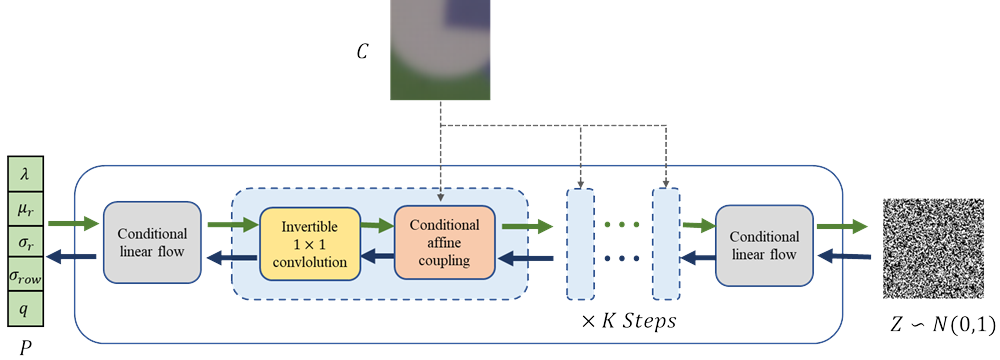
\includegraphics[width=1.0\textwidth]{imgs/parameterflow.pdf}
	\caption{本文提出的用于生成噪声参数的标准化流模型结构。}
	\label{fig:parameterflow}
\end{figure}

给定一个观测到的干净图像数据集$\mathcal{C}=\left\{C_i\right\}_{i=1}^M$和相应的校准噪声参数$\mathcal{P}=\left\{\boldsymbol{P}_i\right\}_{i=1}^M$,其中$M$是数据集的大小。噪声参数$\boldsymbol{P}_i$首先通过条件线性流(Conditional Linear Flow,CLF)层映射为线性变换。在随后的模型中,可逆的$1\times1$卷积层和条件仿射耦合(Conditional Affine Coupling,CAC)层交替使用$K$次。其中,干净的图像作为条件信息进入CAC层作为条件信息。详细的流模型结构将会在下文叙述。模型最后得到的$z$是一个服从标准高斯分布的分布。

上文所叙述的噪声参数流模型可以用式\ref{nllloss}中的负对数似然损失函数进行训练。本文所提出的技术可视为基于流模型的噪声参数先验,它利用标准化流模型的生成能力,从简单分布中提取噪声参数采样。一旦噪声参数流模型经过预训练,参数采样可以通过$\boldsymbol{P}=f_{\boldsymbol{\theta}}^{-1}(\boldsymbol{z})$从高斯分布中采样来生成,其中$\boldsymbol{z} \sim \mathcal{N}(\mathbf{0}, \mathbf{I})$。

\subsection{条件线性流}

由于真实场景中的噪声依赖于图像信号,噪声参数流模型使用条件线性流层来考虑噪声生成的条件信息,包括相机类型$\boldsymbol{t}$及其ISO水平$\boldsymbol{g}$。CLF的结构如图\ref{fig:clf}所示。

\begin{figure}[h]
	\centering
	\includegraphics[width=0.7\textwidth]{imgs/clf.pdf}
	\caption{条件线性流层的结构。}
	\label{fig:clf}
\end{figure}

CLF的数学公式可以表示为:
\begin{equation}
	\boldsymbol{y}=\boldsymbol{x} \odot f_s(\boldsymbol{t}, \boldsymbol{g})+f_t(\boldsymbol{t}, \boldsymbol{g})
\end{equation}
其中$\boldsymbol{x}$和$\boldsymbol{y}$是该层的输入和输出特征图,$\odot$表示点积,$f_s$和$f_t$是计算尺度和平移因子的函数。则该层的逆过程可由下式计算:
\begin{equation}
	\boldsymbol{x}=\left(\boldsymbol{y}-f_t(\boldsymbol{t}, \boldsymbol{g})\right) \oslash f_s(\boldsymbol{t}, \boldsymbol{g})
	\label{clf}
\end{equation}
其中$\oslash$是点除符号。

\subsection{条件仿射耦合}

耦合层必须改变维度在层之间排列的方式,如果维度耦合的顺序保持不变,那么最后的结果依然是平凡的,简单的耦合使得矩阵的其中一部分仍然保持恒等,信息没有充分混合。在NICE模型中是对各个向量进行简单反转\cite{nice},RealNVP模型则是随机打乱\cite{realnvp},而Glow模型引入了使用$1 \times 1$卷积作为可逆变换\cite{glow},可以使模型训练的损失函数收敛到更小的值。在本文提出的模型中,借用Glow模型的思想,条件仿射耦合层将和$1 \times 1$可逆卷积层交替使用,确保信息充分混合。

为了进一步利用信号信息的相关性,标准仿射耦合层\cite{realnvp}被扩展为条件仿射耦合层,将条件信息以及干净图像都作为输入。图\ref{fig:cac}显示了条件仿射耦合层的架构:

\begin{figure}[h]
	\centering
	\includegraphics[width=0.8\textwidth]{imgs/cac.pdf}
	\caption{条件仿射耦合层的结构。}
	\label{fig:cac}
\end{figure}

条件仿射耦合层可以表示为:
\begin{equation}
	\boldsymbol{y}=\boldsymbol{x} \odot f_{c s}(\boldsymbol{x} \mid \boldsymbol{c}, \boldsymbol{t}, \boldsymbol{g})+f_{c t}(\boldsymbol{x} \mid \boldsymbol{c}, \boldsymbol{t}, \boldsymbol{g})
\end{equation}
其中,$\boldsymbol{x}$和$\boldsymbol{y}$是层的输入和输出特征图,$f_{cs}$和$f_{ct}$是使用干净图像$\boldsymbol{c}$、相机类型$\boldsymbol{t}$和ISO水平$\boldsymbol{g}$的来计算缩放和平移的函数。条件仿射耦合层的逆过程可以类似地以式\ref{clf}的形式导出。



\section{基于参数先验的噪声建模}

\subsection{模型整体架构}

有了预先训练的流模型作为噪声参数先验,噪声参数的采样空间就可以大大缩小,进而提高噪声建模的精度。图\ref{fig:noisemodeling}展示了本文噪声建模方法的结构。

\begin{figure}[h]
	\centering
	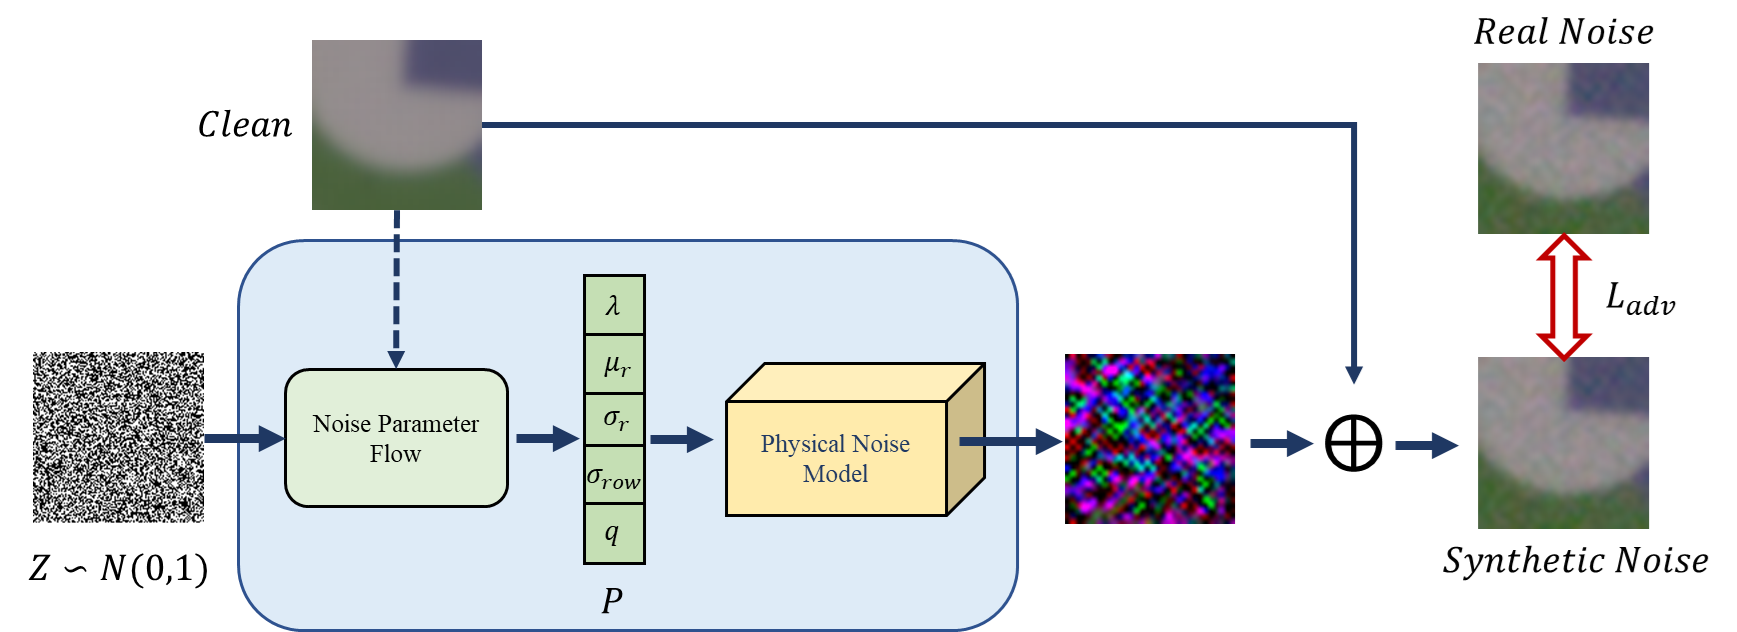
\includegraphics[width=1.0\textwidth]{imgs/noisemodeling.pdf}
	\caption{本文提出的噪声建模方法的结构。}
	\label{fig:noisemodeling}
\end{figure}

本文的工作从一个从高斯分布中随机采样的潜变量$\boldsymbol{z} \sim \mathcal{N}(\mathbf{0}, \mathbf{I})$开始,经过预先训练的噪声参数先验模型获取五个噪声参数$\boldsymbol{P}=\left(\lambda, \mu_r, \sigma_r, \sigma_{\text {row }}, q\right)$。通过获取噪声参数,生成的噪声可通过式\ref{noisemodel}中的物理噪声模型合成,将其添加到干净图像$C$中,得到模型合成的噪声图像$\hat{I}$。

\subsection{损失函数设计}

类似FKP模型,本文采用对抗训练来判别合成的噪声图像是否与真实世界场景足够相似。为了更好地提取噪声图像的特征,本文使用了PatchGAN架构\cite{patchgan}作为对抗训练的判别器,引入了一种稳健的度量方法,包括图像清晰度和结构相似性作。整个模型的优化通过对抗损失函数进行优化:
\begin{equation}
	\mathcal{L}_{a d v}=-\mathbb{E}_I[\log D(I)]-\mathbb{E}_{\boldsymbol{z}}[\log (1-D(G(\boldsymbol{z})))]
\end{equation}
其中$I$是真实捕获的噪声图像。

在噪声建模训练过程中,由于预训练的噪声参数流模型是固定的,因此实际优化参数是潜变量$\boldsymbol{z}$。通过搜索最优的潜变量$\boldsymbol{z}$,可以找到对于特定数据集最合适的噪声参数。在噪声生成阶段,有了优化的$\boldsymbol{z}$和干净的图像$C$,可以通过预训练的噪声参数流模型生成大量的噪声图像。通过结合基于流的参数先验,所提出的噪声建模方法可以根据特定的相机传感器适应各种物理噪声模型,有助于提高图像去噪质量。



\chapter{实验结果与分析}
\section{实验设置}

\noindent\textbf{数据集选择} \quad 根据该领域此前最先进的噪声模型Noise Flow\cite{noiseflow}、FGNM\cite{co},该领域最为广泛使用的数据集为智能手机图像去噪数据集(Smartphone Image Denoising Dataset,SIDD)\cite{sidd},因此本文同样选择SIDD数据集来评估本文提出的方法的性能。SIDD数据集包含320个噪声干净RAW图像对,这些图像对在不同的ISO水平和照明条件下,由5个不同的智能手机拍摄,包含10个不同的场景。ISO水平的范围是50到10000。与此同时,该数据集提供了一个简化的ISP图像处理管道,用于将图像从RAW域渲染到sRGB域,如下图所示:

\begin{figure}[htbp]
	\centering
	\begin{subfigure}{0.48\linewidth}
		\centering
		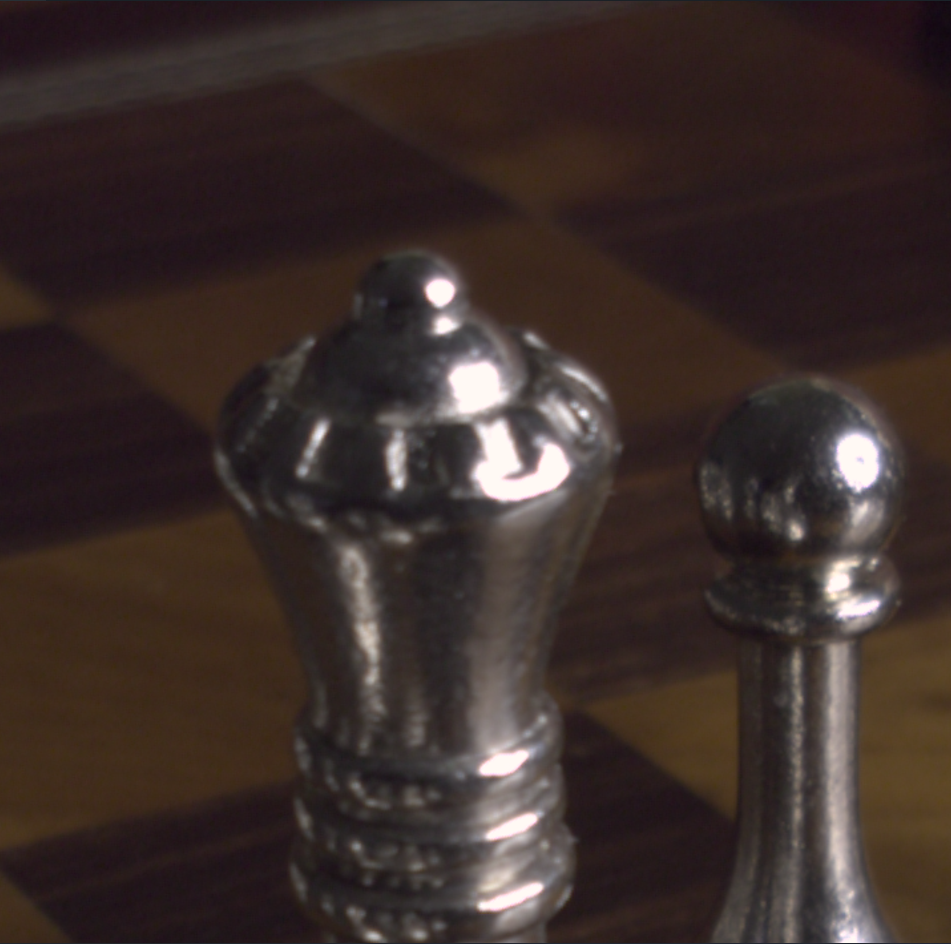
\includegraphics[width=\linewidth]{imgs/gtcut.png}
		\caption{干净图像}
		\label{gt}%文中引用该图片代号
	\end{subfigure}
	\centering
	\begin{subfigure}{0.4835\linewidth}
		\centering
		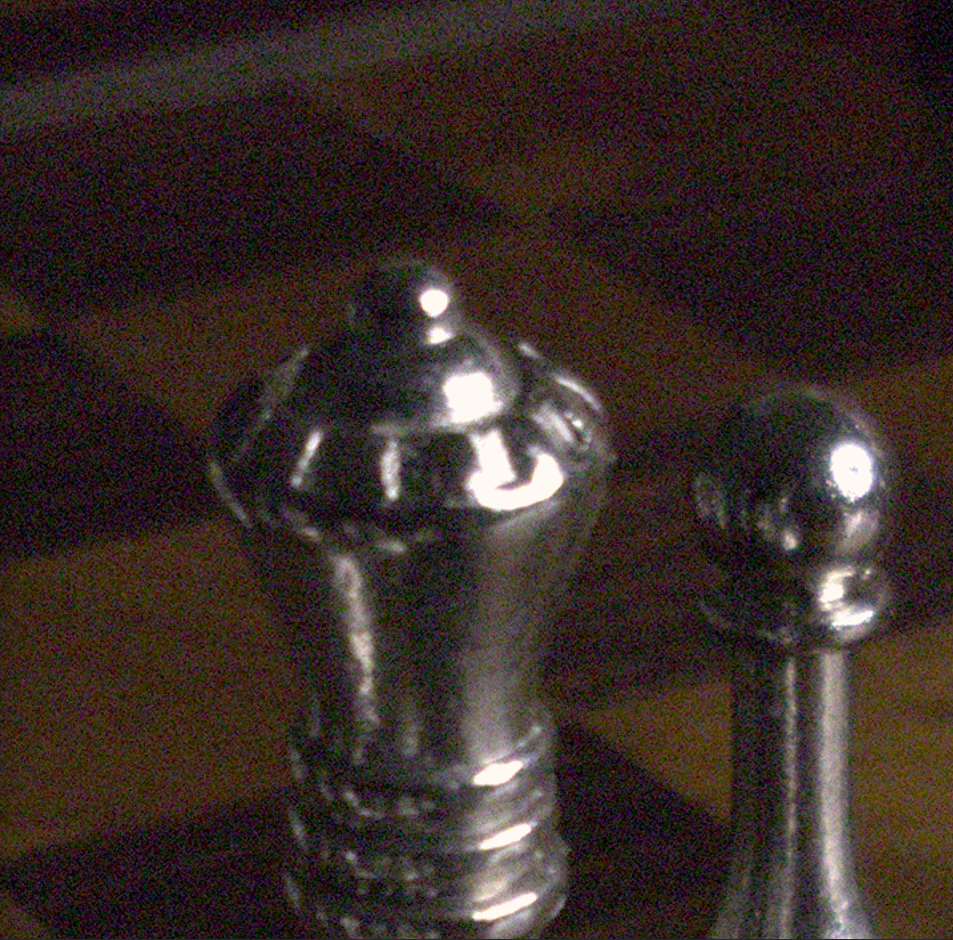
\includegraphics[width=\linewidth]{imgs/noisycut.png}
		\caption{噪声图像}
		\label{noisy}%文中引用该图片代号
	\end{subfigure}  
	
	\caption{SIDD中的干净-噪声图像对}
\end{figure}

在本文评估去噪性能的时候,还采用了极端低光去噪数据集(Extreme Low-light Denoising,ELD)\cite{eld}。ELD数据集包括10种不同的场景,由4种来自不同品牌的相机拍摄。该数据集选择了多种不同的拍摄设置,共产生了240个RAW图像对。

\begin{figure}[htbp]
	\centering
	\begin{subfigure}{0.49\linewidth}
		\centering
		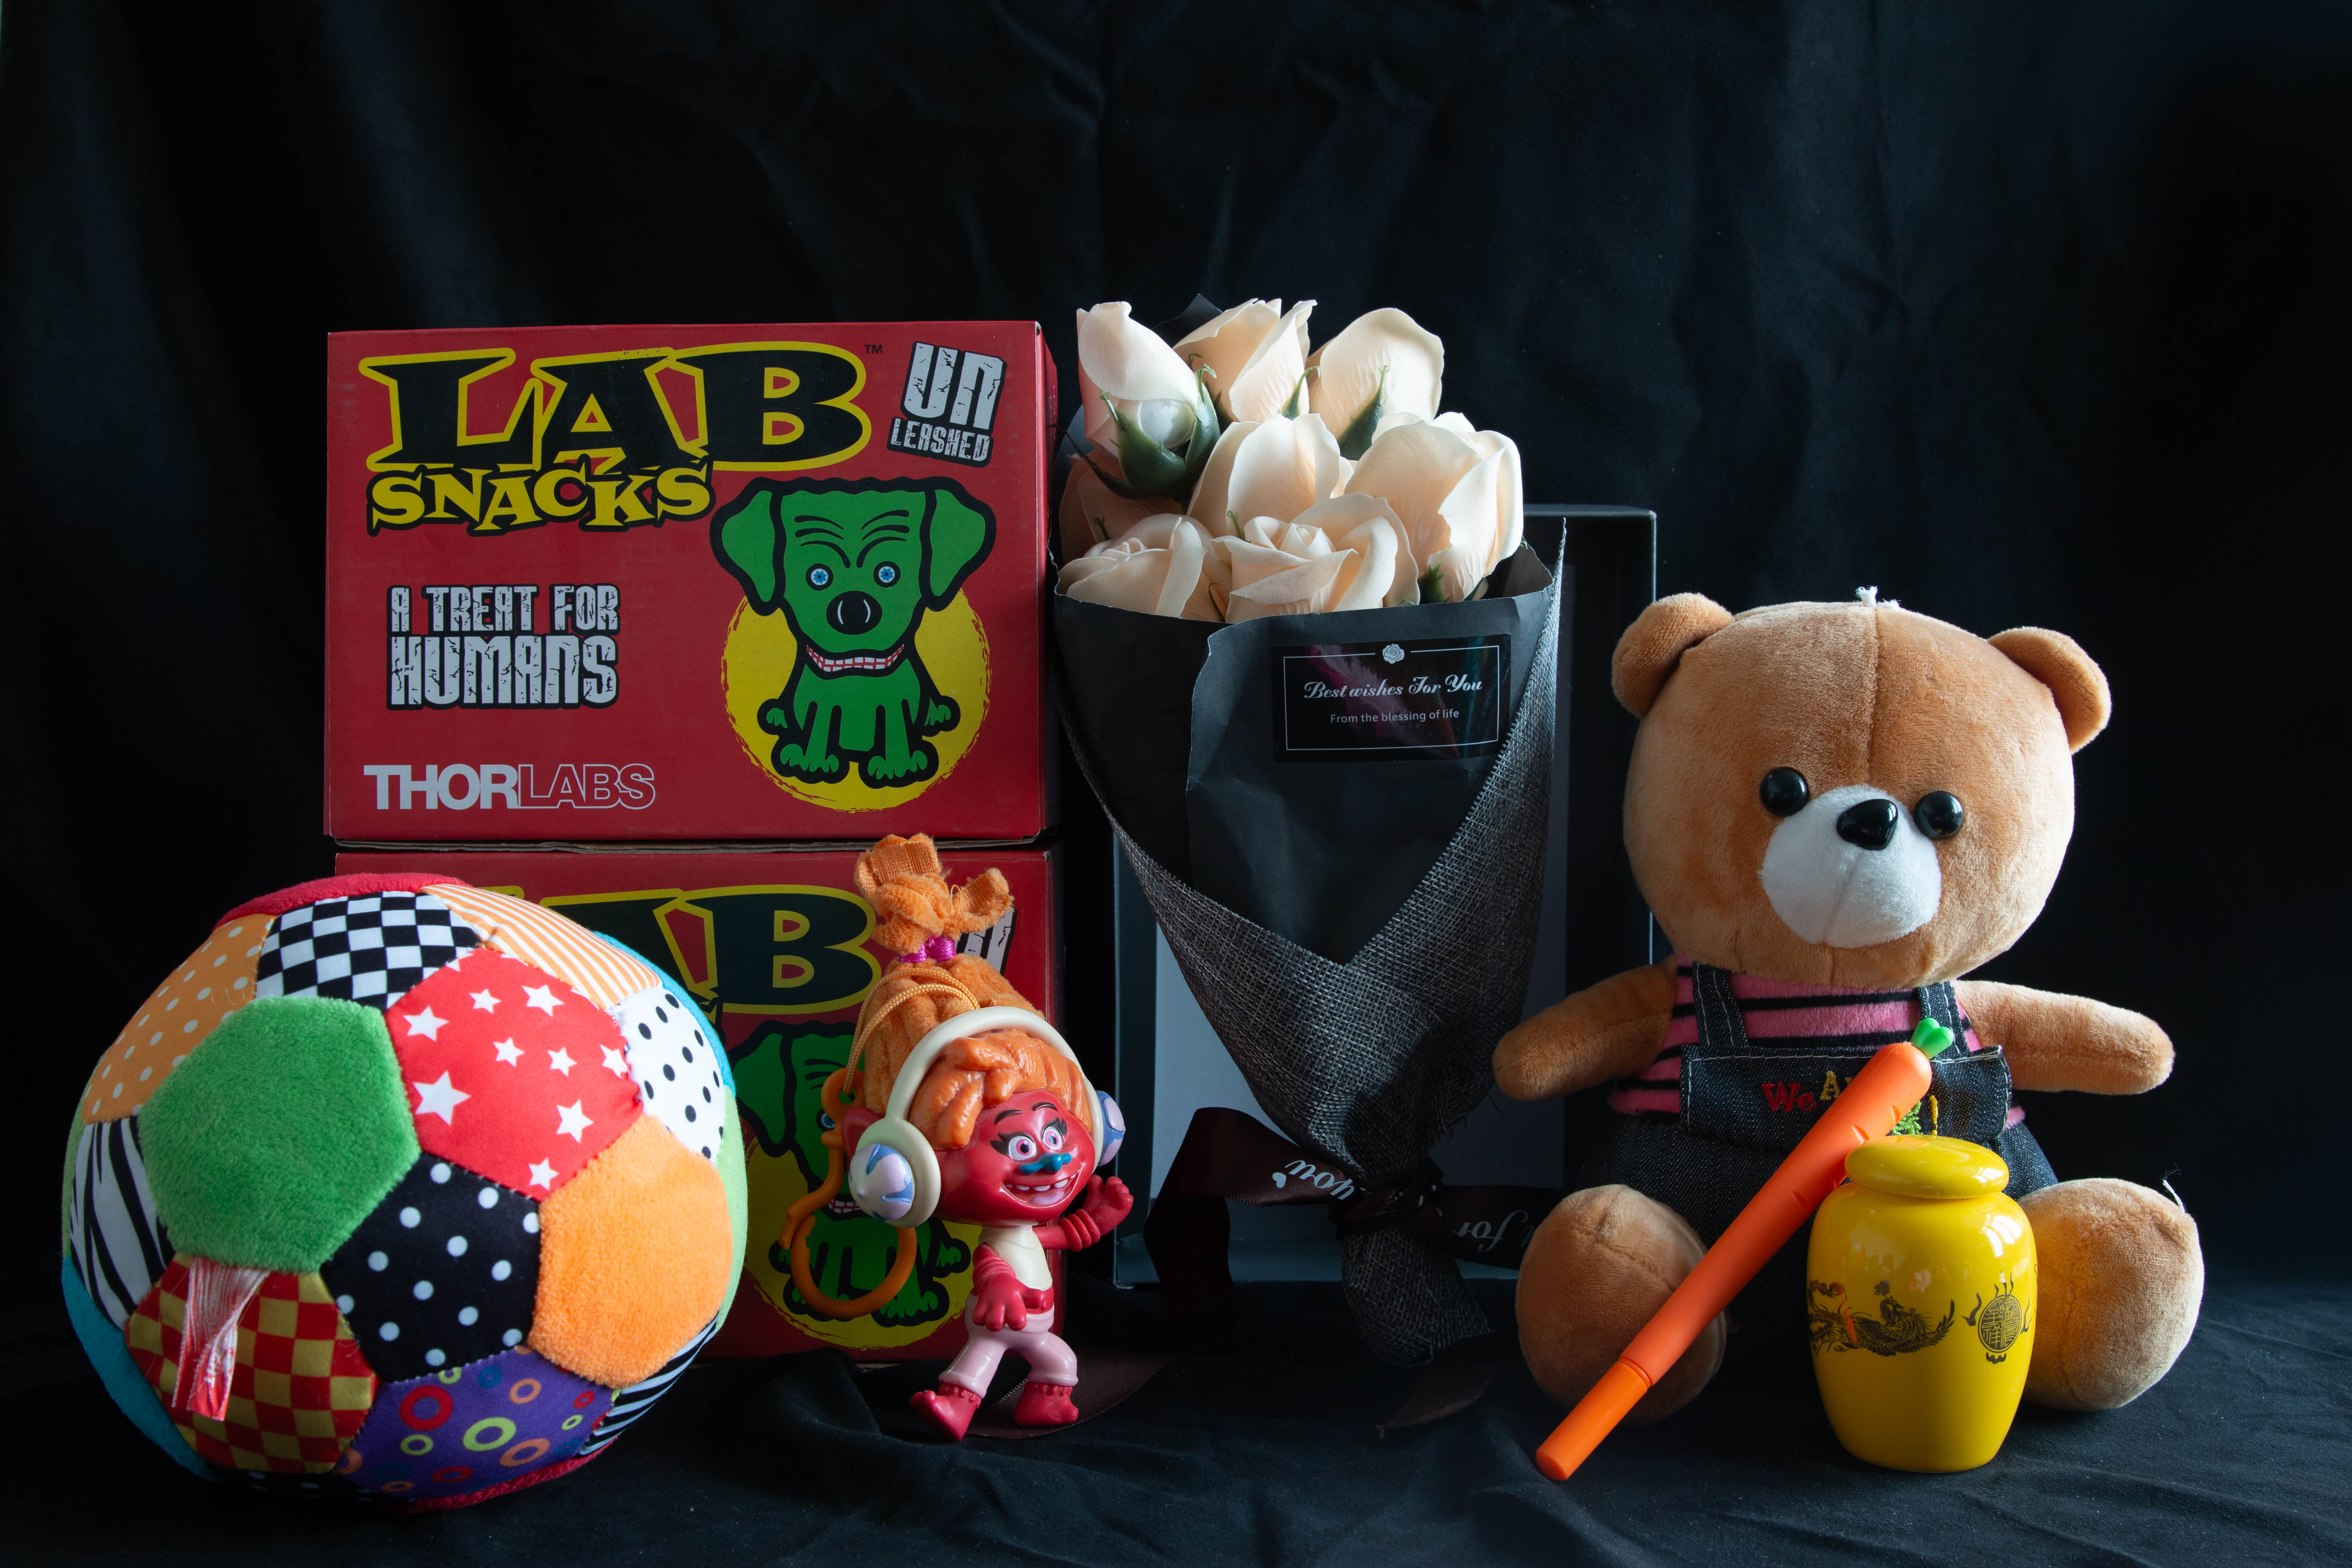
\includegraphics[width=\linewidth]{imgs/ELD1.jpg}
		
		\label{eld1}%文中引用该图片代号
	\end{subfigure}
	\centering
	\begin{subfigure}{0.49\linewidth}
		\centering
		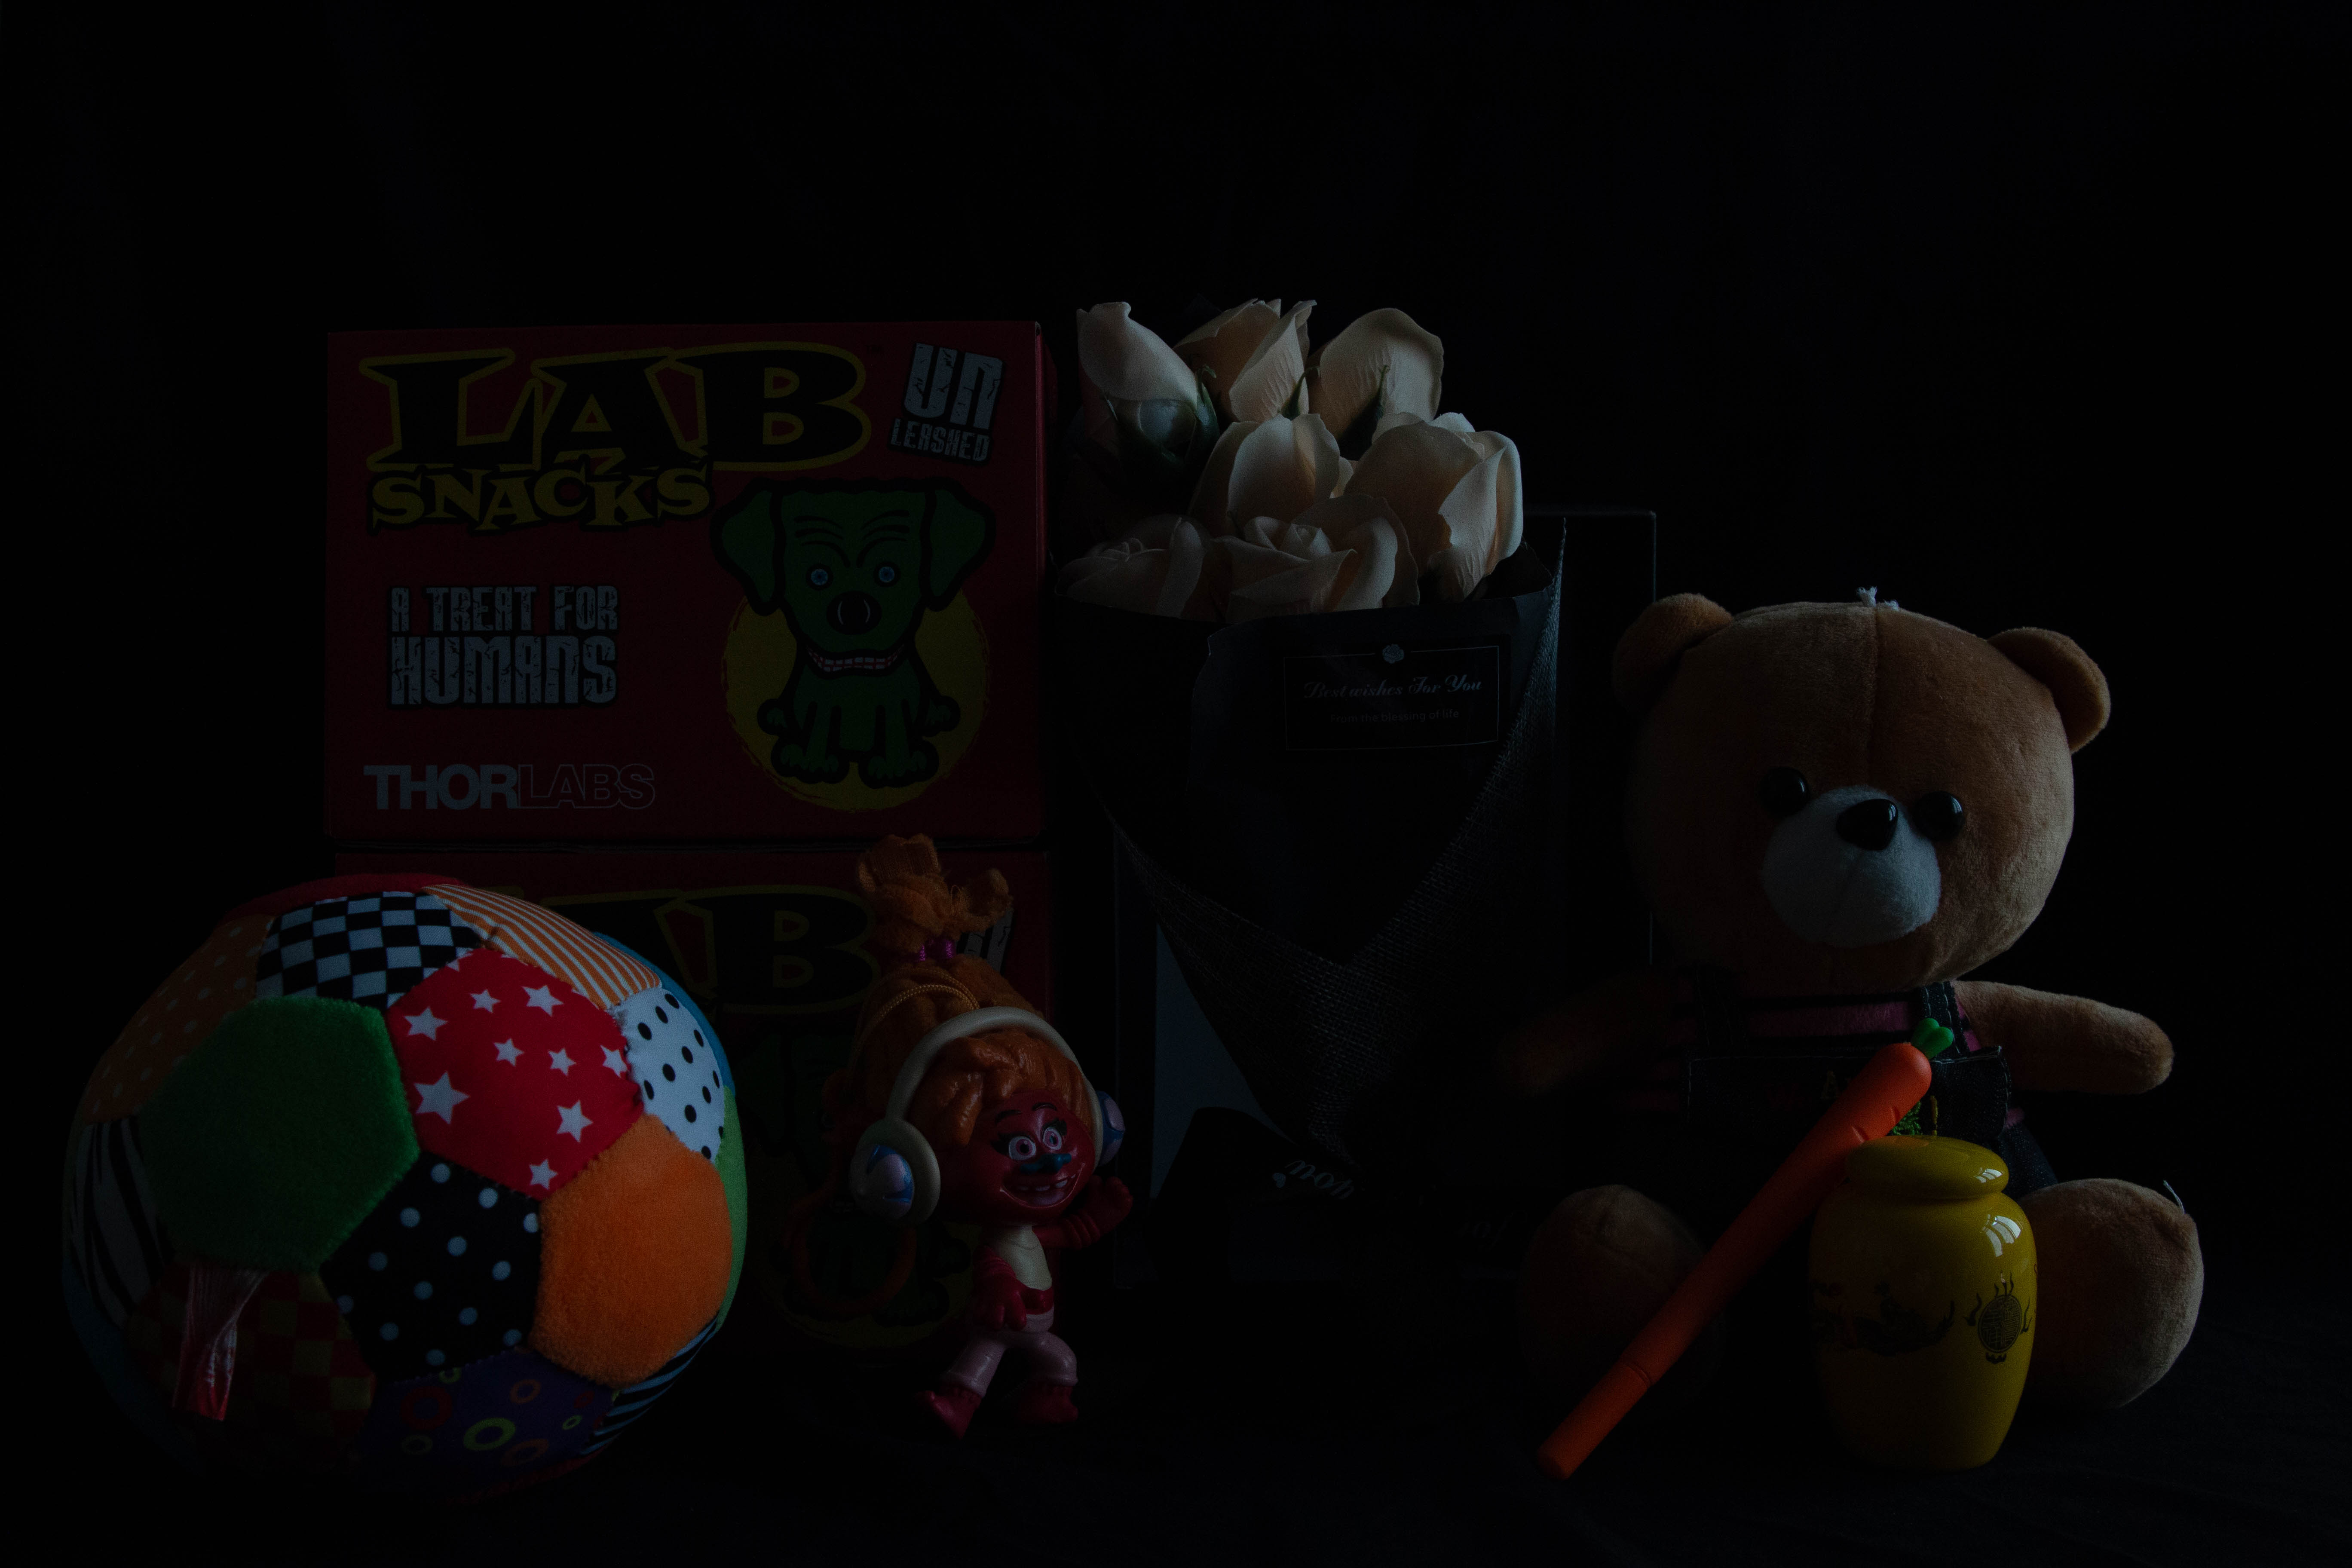
\includegraphics[width=\linewidth]{imgs/ELD3.jpg}
		
		\label{eld3}%文中引用该图片代号
	\end{subfigure}  
	
	\caption{ELD中同一场景下不同拍摄设置拍摄出的照片}
\end{figure}

\noindent\textbf{评估指标} \quad 为了定量评估性能,本文在对比时使用最常用的评估指标。对于噪声合成,为了评估合成噪声和真实捕获噪声之间的相似性,本文应用Kullback-Leibler (KL)散度来衡量两个分布之间的差异。KL散度的公式为:
\begin{equation}
	D_{K L}(p \| q)=\sum_{i=1}^n p(x) \log \frac{p(x)}{q(x)}
\end{equation}

对于真实去噪性能,本文使用峰值信噪比(Peak Signal-to-Noise Ratio,PSNR)作为指标之一,PSNR是基于均方误差(Mean Square Error,MSE)来定义的,给定一个大小为$m \times n$的原始图像$I$和经过处理的图像$K$,其MSE可定义为:
\begin{equation}
	M S E=\frac{1}{m n} \sum_{i=0}^{m-1} \sum_{j=0}^{n-1}[I(i, j)-K(i, j)]^2
\end{equation}
则PSNR可定义为:
\begin{equation}
	PSNR=20 \cdot \log _{10}\left(\frac{M A X_I}{\sqrt{M S E}}\right)
\end{equation}
其中$M A X_I$为图像的最大像素值。

此外,本文还使用结构相似性(Structural Similarity,SSIM)来作为两幅图像相似度的指标。SSIM由三个部分组成:亮度(luminance)、对比度(contrast)和结构(structure)。SSIM通过滑动窗口实现,遍历整张图像后将所有窗口的数值取平均值作为整张图像的SSIM指标。假设$x$、$y$分别表示两张图像窗口中的数据,亮度的计算公式为:
\begin{equation}
	l(x, y)=\frac{2 \mu_x \mu_y+c_1}{\mu_x^2+\mu_y^2+c_1}
\end{equation}
对比度的计算公式为:
\begin{equation}
	c(x, y)=\frac{2 \sigma_x \sigma_y+c_2}{\sigma_x^2+\sigma_y^2+c_2}
\end{equation}
结构的计算公式为:
\begin{equation}
	s(x, y)=\frac{\sigma_{x y}+c_3}{\sigma_x \sigma_y+c_3}
\end{equation}
其中$\mu$表示均值,$\sigma$表示方差,$c$表示常数,最后SSIM的计算公式为:
\begin{equation}
	SSIM(x, y)=\left[l(x, y)^\alpha \cdot c(x, y)^\beta \cdot s(x, y)^\gamma\right]
\end{equation}
参数$\alpha$、$\beta$、$\gamma$通常取1。

\noindent\textbf{数据增强} \quad 在现有噪声参数的基础上,本文采用了一种有价值的数据增强策略,即在参数中添加方差为$0.1$的高斯扰动。这项技术通过引入方差作为附加信息,丰富了有限的数据集,有助于提高生成模型的鲁棒性。数据集的这种微小但有意义的变化可以与本文预训练的标准化流模型无缝集成,展示了一种增强的噪声建模方法。此外,它还允许模型考虑不可预测的真实世界变化,从而提高了神经网络噪声建模能力的准确性和有效性。


\noindent\textbf{实现细节} \quad 本文的模型训练设置效仿了Noise Flow模型\cite{noiseflow},使用Adam优化器进行训练,迭代20万次。初始学习率为0.0002,学习率调整使用余弦退火算法。模型训练并不会使用整张图片,而是将图片切成$64\times 64$的块,同时一次迭代会处理16个样本。

\section{实验结果}



\subsection{噪声建模的对比}

为了评估所提出的噪声建模方法的噪声合成性能,本文将合成噪声和真实噪声之间的KL散度与几种最先进的噪声建模方法进行了比较。
\begin{table*}[htbp]
	\begin{center}
		\tabcolsep = 1.7cm
		\caption{不同噪声建模方法在SIDD数据集上的平均KL散度表现(越小越好)}
		\label{compareNoise}
		\begin{tabular}{c|c}
			\toprule[1.5pt]
			方法 & 平均KL散度\\
			\midrule [1pt]
			AWGN & 0.7544\\
			P-G \cite{foi2008noise} & 0.0467\\
			Noise Flow \cite{noiseflow} & 0.0590 \\
			CANGAN \cite{learningcamera} & 0.0220\\
			FGNM \cite{co}& 0.0211\\
			\midrule[1pt]
			本文的模型& \textbf{0.0188}\\
			
			\bottomrule[1.5pt]
		\end{tabular}
	\end{center}
\end{table*}

平均KL散度的比较如表\ref{compareNoise}所示。参与比较的基准方法包括参数化噪声模型(即加性高斯白噪声模型和泊松-高斯噪声模型\cite{foi2008noise})和基于深度学习的噪声模型(即Noise Flow\cite{noiseflow}、CANGAN\cite{learningcamera}和FGNM\cite{co})。

可以看到,在参数化噪声建模方法中,AWGN模型的性能最差,P-G噪声模型由于包含了信号依赖性,更适合于模拟真实噪声。深度学习方法Noise Flow\cite{noiseflow}由于其训练的不稳定性,性能略逊于P-G。本文提出的方法获得了最佳的KL散度表现,证明了优越性。

各种噪声建模方法合成噪声图像的比较如图\ref{fig:compareNoise}所示,图中展示了来自不同ISO水平(100到1600)和光照条件的样本(N:正常光,L:暗光)。

\begin{figure}[h]
	\centering
	\includegraphics[width=1.0\textwidth]{imgs/compareNoise.pdf}
	\caption{ISO水平和照明条件(N:正常光,L:暗光)显示在左侧,KL散度显示在图像块左上角,这些RAW图像块通过SIDD提供的ISP处理管线进行可视化}
	\label{fig:compareNoise}
\end{figure}

本文在图\ref{viscom1}和\ref{viscom2}中展示了SIDD数据集上的更多可视化结果。可以看出,本文的方法生成的噪声图像在视觉上比其他方法更接近于真实的噪声分布,KL散度也定量地证明了这点,体现了本文所提出的方法在噪声建模任务中的优越性。

\begin{figure}[htbp]
	\centering
	\begin{subfigure}{\linewidth}
		\centering
		\includegraphics[width=0.73\linewidth]{imgs/viscom1.pdf}
		\caption{}
		\label{viscom1}%文中引用该图片代号
	\end{subfigure}
	\centering
	\begin{subfigure}{\linewidth}
		\centering
		\includegraphics[width=0.73\linewidth]{imgs/viscom2.pdf}
		\caption{}
		\label{viscom2}%文中引用该图片代号
	\end{subfigure}  
	
	\caption{不同噪声模型合成的噪声图像对比}
\end{figure}

\subsection{真实图像去噪}

为了进一步证明所提出方法的噪声生成能力,本文使用不同的噪声建模方法来生成成对的噪声-干净样本并训练RAW图像去噪网络。通过评估真实噪声图像上的去噪性能,可以进一步比较噪声先验学习的准确性。采用Noise Flow\cite{noiseflow}的实验思路,本文使用在相关工作介绍过的的标准DnCNN网络\cite{dncnn}作为去噪网络,包含10个卷积层。

ELD数据集上的去噪结果如表\ref{dncnneld}所示,可以看出,以本文的模型作为噪声先验训练的DnCNN模型在PSNR和SSIM指标上取得了显著更高的性能。

\begin{table}[h]
	\centering
	\caption{对比不同噪声先验DnCNN以及盲去噪方法Nois2Noise在ELD数据集上的表现}
	\label{dncnneld}
	\begin{subtable}{\linewidth}
		\centering
		\caption{PSNR}
		\resizebox{\textwidth}{!}{
			\begin{tabular}{c|c|ccccc}
				\toprule[1.5pt]  
				相机型号 &  快门速度(s) & Gaussian  & P-G\cite{foi2008noise} &  Noise2Noise\cite{noise2noise} & 真实噪声 & 本文的模型 \\
				\midrule[1pt]  
				\multirow{2}{*}{Sony A7S2} & $1/400$ & 42.35 & 42.46 & 41.63 & 44.50 & \textbf{45.49} \\
				& $1/800$ & 38.93 & 38.88 & 37.98 & 42.45 & \textbf{43.37} \\
				\midrule[1pt]			               
				\multirow{2}{*}{Nikon D850} & $1/400$ & 39.57 & 40.29 & 40.47 & 41.28 & \textbf{42.17} \\
				& $1/800$ & 36.68 & 37.26 & 37.98 & 39.44 & \textbf{39.98}\\
				\midrule[1pt]
				\multirow{2}{*}{Canon EOS70D} &$1/400$& 40.59 & 40.94 & 38.21 & 41.10 &\textbf{ 41.17}\\
				&$1/800$& 37.49 & 37.64 & 34.33 & 37.32 & \textbf{38.26}\\
				\midrule[1pt]		                  
				\multirow{2}{*}{Canon EOS700D}&$1/400$& 39.77 & 40.08 & 38.29 & 39.05 & \textbf{40.07}\\
				&$1/800$& 37.67 & 37.86 & 34.94 & 36.50 & \textbf{37.56}\\
				\bottomrule[1.5pt]
			\end{tabular}
		}
	\end{subtable}
	
	\begin{subtable}{\linewidth}
		\centering
		\caption{SSIM}
		\resizebox{\textwidth}{!}{
			\begin{tabular}{c|c|ccccc}
				\toprule[1.5pt]  
				相机型号 &  快门速度(s) & Gaussian  & P-G\cite{foi2008noise} &  Noise2Noise\cite{noise2noise} & 真实噪声 & 本文的模型 \\
				\midrule[1pt]  
				\multirow{2}{*}{Sony A7S2} & $1/400$ & 0.893 & 0.889 & 0.856 & 0.971 & \textbf{0.982} \\
				& $1/800$ & 0.813 & 0.812 & 0.775 & 0.945 & \textbf{0.952} \\
				\midrule[1pt]			               
				\multirow{2}{*}{Nikon D850} & $1/400$ & 0.823 & 0.845 & 0.848 & 0.938 & \textbf{0.947}  \\
				& $1/800$ & 0.757 & 0.786 & 0.820 & \textbf{0.910} & 0.899 \\
				\midrule[1pt]
				\multirow{2}{*}{Canon EOS70D} &$1/400$& 0.925 & 0.934 & 0.826 & 0.931 & \textbf{0.947} \\
				&$1/800$& 0.871 & 0.873 & 0.704 & 0.867 & \textbf{0.895} \\
				\midrule[1pt]		                  
				\multirow{2}{*}{Canon EOS700D}&$1/400$& 0.884 & 0.897 & 0.859 & 0.906 & \textbf{0.913} \\
				&$1/800$& 0.870 & 0.879 & 0.766 & 0.850 & \textbf{0.896} \\
				\bottomrule[1.5pt]
			\end{tabular}
		}
	\end{subtable}
	
\end{table}

值得注意的是,本文的噪声建模方法提供了更多的训练样本,因此与真实噪声先验相比,以本文的模型作为噪声先验训练的DnCNN网络可以获得相似或更高的结果。

SIDD数据集上本文的模型表现仍然优异,表\ref{dncnnsidd}展示了PSNR指标的定量分析,图\ref{fig:dncnnsidd}展示了视觉效果的对比,本文的模型都取得了最好或仅次于真实噪声先验的效果。

\begin{table}[htbp]
	\begin{center}
		
		\caption{对比不同噪声先验DnCNN在SIDD数据集上的表现}
		\label{dncnnsidd}
		\begin{tabular}{c|cccc}
			\toprule[1.5pt]
			方法 & 400-L & 400-N & 800-L & 800-N \\
			\midrule[1pt]
			Gaussian & 43.79 & 52.20 & 56.59 & 49.94 \\
			Noise Flow\cite{noiseflow} & 47.79 & 56.03 & 56.64 & 50.72 \\
			DnCNN-Real & 44.21 & 57.94 & \textbf{57.10} & 49.41 \\
			\midrule[1pt]
			本文的模型 & \textbf{48.24} & \textbf{58.21} & 56.79 & \textbf{50.98} \\
			\bottomrule[1.5pt]
		\end{tabular}
	\end{center}
\end{table}

\begin{figure}[h]
	\centering
	\includegraphics[width=1.0\textwidth]{imgs/dncnnsidd.pdf}
	\caption{不同噪声先验的视觉去噪效果}
	\label{fig:dncnnsidd}
\end{figure}

\section{消融实验}

为了验证所提出方法的有效性,本文进行了两项消融研究。本文消融了预训练的噪声先验以及数据增强策略,消融结果如表\ref{ablation}所示。表中本文提出的基于流模型的噪声参数先验(Flow-based Parameter Prior)简称为FPP,数据增强(Data Augmentation)简称为DA。表中比较了不同变体的PSNR和SSIM结果,可以看到,在预训练了基于流的参数先验后,由于噪声建模更加精确,去噪结果得到了显著改善。数据增强策略也能带来更高的结果。

\begin{table}[h]
	\begin{center}
		\caption{消融实验的结果}
		\label{ablation}
		\begin{tabular}{cc|cc|cc|cc|cc}
			\toprule[1.5pt]
			\multirow{2}{*}{FPP} & \multirow{2}{*}{DA} & \multicolumn{2}{c|}{ Sony A7S2 } & \multicolumn{2}{c|}{ Nikon D850 } & \multicolumn{2}{c|}{ Canon EOS70D } & \multicolumn{2}{c}{ Canon EOS700D } \\
			& & 1/400 & 1/800 & 1/400 & 1/800 & 1/400 & 1/800 & 1/400 & 1/800 \\
			\midrule[1pt]
			
			\multirow{2}{*}{$\checkmark$} & & 45.10 & 42.53 & 41.93 & 38.10 & 40.06 & 37.99 & 39.37 & 36.02 \\
			& & 0.978 & 0.947 & 0.921 & 0.884 & 0.938 & 0.825 & 0.869 & 0.899 \\
			\midrule[1pt] 
			
			& \multirow{2}{*}{$\checkmark$} & 45.06 & 42.10 & 41.26 & 37.63 & 39.76 & 37.94 & 39.52 & 35.47 \\
			& & 0.974 & 0.938 & 0.932 & 0.874 & 0.919 & 0.825 & 0.886 & 0.875 \\
			\midrule[1pt] 
			
			\multirow{2}{*}{$\checkmark$} & \multirow{2}{*}{$\checkmark$} & 45.49 & 43.37 & 42.17 & 39.98 & 41.17 & 38.26 & 40.07 & 37.56 \\
			& & 0.982 & 0.952 & 0.947 & 0.899 & 0.947 & 0.895 & 0.913 & 0.896 \\
			\bottomrule[1.5pt]
		\end{tabular}
	\end{center}
\end{table}
\chapter{总结与展望}
\section{本文总结}

本文提出了一种创新的噪声先验学习方法,称为基于流模型的噪声参数先验。这种方法充分利用预训练的噪声参数流模型,以简单的高斯分布表示复杂的噪声参数场,极大缩小了物理噪声参数的采样空间。与传统噪声建模方法不同,本文的方法并不直接合成复杂的噪声,而是先从潜在空间生成噪声参数,再通过物理噪声模型生成最终的噪声,从而提高了噪声建模的精确性和可靠性。通过对抗训练,本文所提出的方法无需依赖成对的噪声-清洁训练数据,这不仅降低了数据获取的难度,还增强了方法的适应性和灵活性。这一先进而灵活的框架可以根据不同的物理参数模型和相机传感器进行调整,为处理不同种类的噪声先验问题提供了全新的解决方案。

本文的技术贡献总结如下:

(1)本文提出了一种新颖的生成式噪声建模方法来进行噪声先验学习。(2)本文的方法显著压缩了物理噪声参数所需的采样空间,提高了建模的计算效率和精度。(3)本文提出的灵活噪声建模框架可以根据不同的物理参数噪声模型进行动态配置。(4)广泛的实验结果表明,本文的噪声先验方法合成的噪声在主观和客观质量方面都达到了最先进的水平,在真实图像去噪应用中展现了显著的优势,不仅显著提高了去噪效果,还显现出该方法在实际应用中的实用性和通用性。

\section{算法展望}

虽然本文提出的方法取得了先进的效果,但仍有可以改进的地方,未来的研究希望进一步提升和扩展本文提出的基于流模型的噪声参数先验方法。首先,通过开发更多样化的预训练模型并整合丰富的先验知识,可以使模型更精确地捕捉多种类型的噪声特征,包括自然噪声和人为引入的噪声。这将使我们能够应对更复杂的噪声建模场景,例如高动态范围成像、低光环境成像、以及特殊的医疗或工业成像应用。

其次,与现有的先进图像传感器和物理噪声模型相结合,可以实现针对特定领域的定制化噪声建模。例如,医疗影像学和航空摄影等领域都依赖于高质量图像,并且面临着独特的噪声挑战,通过定制的噪声建模框架可以更有效地满足这些领域的需求。

此外,将该方法中的生成模型换成其他更先进的生成模型(例如扩散模型)也将是一个有前景的方向。更先进的生成模型有望提供更高效、更逼真的图像噪声建模,使其在更广泛的领域发挥作用。


\end{document}